\documentclass[10pt,a4paper]{article}

\usepackage[a4paper,margin=1.2cm]{geometry}
\usepackage{fontspec}
\setmainfont{Latin Modern Mono}

\usepackage{emoji}
\setemojifont{Apple Color Emoji}

\usepackage[activeacute]{babel}
\usepackage{polyglossia}
\setotherlanguages{hebrew}
\newfontfamily{\hebrewfont}[Script=Hebrew]{Hadasim CLM}
\newfontfamily{\hebrewfontsf}[Script=Hebrew]{Miriam CLM}
\newfontfamily{\hebrewfonttt}[Script=Hebrew]{Miriam Mono CLM}

\usepackage{fontawesome5}
\usepackage{paracol}
\usepackage{xcolor}
\usepackage{tcolorbox}
\tcbuselibrary{listings,skins,breakable}
\usepackage{listings}
\usepackage{CJKutf8,luatexja-fontspec}
\usepackage{pagecolor}
\usepackage{tikz}
\usetikzlibrary{arrows,calc,decorations.pathmorphing,positioning,patterns}
\usepackage{tikz-feynman}
\usepackage{graphicx}
\usetikzlibrary{overlay-beamer-styles}
\usepackage{eso-pic}
\usepackage{physics}
\usepackage{chemfig}
\usepackage{hyperref}
\hypersetup{
  colorlinks=true,
  linktoc=all,
  linkcolor=darkblue,
  citecolor=antiquefuchsia,
  urlcolor=darkblue,
  pdfauthor={VCastor},
  pdftitle={CV}
}


% ---------
% Colours
% ---------
\definecolor{terminalgreen}{RGB}{0, 150, 0}
\definecolor{terminalgray}{RGB}{220, 220, 215} 
\definecolor{terminalwhite}{RGB}{30, 30, 30}
\definecolor{terminalcyan}{RGB}{0, 130, 180}
\definecolor{terminalprompt}{RGB}{60, 130, 0}
\definecolor{macred}{RGB}{255, 95, 86} 
\definecolor{macyellow}{RGB}{255, 189, 68} 
\definecolor{macgreen}{RGB}{39, 201, 63}
\definecolor{pagebg}{RGB}{255, 255, 255}
\definecolor{darkblue}{RGB}{30, 60, 140}
\definecolor{textmain}{RGB}{30, 30, 30}
\definecolor{terminalblack}{RGB}{250, 250, 248}
\definecolor{windowbg}{RGB}{242, 242, 235}
% \definecolor{windowbg}{RGB}{250, 250, 248}
\definecolor{terminalyellow}{RGB}{70, 90, 150}
\definecolor{terminalred}{RGB}{45, 110, 180}
\definecolor{framegray}{RGB}{210, 210, 210}
\definecolor{frameborder}{RGB}{190, 190, 190}

% Set page background
\pagecolor{pagebg}

% TikZ helper commands for magnetic field
\newcommand\pgfmathsinandcos[3]{%
  \pgfmathsetmacro#1{sin(#3)}%
  \pgfmathsetmacro#2{cos(#3)}%
}
\newcommand\LongitudePlane[3][current plane]{%
  \pgfmathsinandcos\sinEl\cosEl{#2}
  \pgfmathsinandcos\sint\cost{#3}
  \tikzset{#1/.estyle={cm={\cost,\sint*\sinEl,0,\cosEl,(0,0)}}}
}
\newcommand\LatitudePlane[3][current plane]{%
  \pgfmathsinandcos\sinEl\cosEl{#2}
  \pgfmathsinandcos\sint\cost{#3}
  \pgfmathsetmacro\yshift{\cosEl*\sint}
  \tikzset{#1/.estyle={cm={\cost,0,0,\cost*\sinEl,(0,\yshift)}}}
}
\newcommand\DrawLongitudeCircle[2][1]{
  \LongitudePlane{\angEl}{#2}
  \tikzset{current plane/.prefix style={scale=#1}}
  \pgfmathsetmacro\angVis{atan(sin(#2)*cos(\angEl)/sin(\angEl))}
  \draw[current plane] (\angVis:1) arc (\angVis:\angVis+180:1);
  \draw[current plane,dashed] (\angVis-180:1) arc (\angVis-180:\angVis:1);
}
\newcommand\DrawLatitudeCircle[2][1]{
  \LatitudePlane{\angEl}{#2}
  \tikzset{current plane/.prefix style={scale=#1}}
  \pgfmathsetmacro\sinVis{sin(#2)/cos(#2)*sin(\angEl)/cos(\angEl)}
  \pgfmathsetmacro\angVis{asin(min(1,max(\sinVis,-1)))}
  \draw[current plane] (\angVis:1) arc (\angVis:-\angVis-180:1);
  \draw[current plane,dashed] (180-\angVis:1) arc (180-\angVis:\angVis:1);
}

%----------------------------
% Terminal / listing styles
%----------------------------

\tcbuselibrary{listings,skins,breakable}

\lstdefinestyle{terminal}{
  backgroundcolor=\color{terminalblack},
  basicstyle=\ttfamily\small\color{terminalgreen},
  keywordstyle=\color{terminalcyan}\bfseries,
  commentstyle=\color{gray!60},
  stringstyle=\color{terminalyellow},
  showstringspaces=false,
  breaklines=true,
  columns=fullflexible,
  keepspaces=true,
  language=bash,
  frameround=tttt,
  framesep=4pt,
  rulecolor=\color{gray!30},
  xleftmargin=5pt,
  xrightmargin=5pt,
  literate={~}{{\textcolor{terminalprompt}{>}}}{1}
           {\$}{{\textcolor{terminalprompt}{\$}}}{1}
           {>}{{\textcolor{terminalprompt}{ }}}{1},
  moredelim={[is][\color{yellow}\bfseries]{@@}{@@}},
  moredelim={[is][\color{red}\itshape]{!!}{!!}},
  moredelim={[is][\color{cyan}\underline]{__}{__}},
}

\lstdefinestyle{termadv}{
  backgroundcolor=\color{windowbg},
  basicstyle=\ttfamily\small\color{textmain},
  moredelim=[l][\color{terminalgreen}\bfseries]{\$},
  moredelim=[l][\color{gray!70}]{>},
  moredelim=[l][\color{terminalprompt}\bfseries]{\#},
  morekeywords={print,name,contact,education,PhD,Master,Bachelor,languages,skills},
  breaklines=true,
  columns=fullflexible,
  keepspaces=true,
  showstringspaces=false,
  tabsize=4,
  escapeinside={§§},
}

\newcommand{\hlline}[1]{\colorbox{yellow!30}{#1}}
\newcommand{\hlerror}[1]{\colorbox{red!20}{#1}}
\newcommand{\hlsuccess}[1]{\colorbox{green!20}{#1}}

\newtcblisting{macterminal}[1][Terminal]{%
  listing only,
  listing options={
    style=termadv,
    aboveskip=0pt,
    belowskip=0pt,
    xleftmargin=0pt,
    xrightmargin=0pt,
    framexleftmargin=0pt,
    framexrightmargin=0pt,
  },
  enhanced,
  colback=windowbg,
  colframe=framegray,
  arc=3pt,
  outer arc=3pt,
  boxrule=1pt,
  left=8pt,
  right=8pt,
  top=20pt,
  bottom=8pt,
  enlarge top initially by=0pt,
  overlay={
    \fill[framegray] 
      ([yshift=-3pt]frame.north west) 
      arc (180:90:3pt)
      -- ([xshift=-3pt]frame.north east)
      arc (90:0:3pt)
      -- ([yshift=-20pt]frame.north east)
      -- ([yshift=-20pt]frame.north west)
      -- cycle;
    \fill[macred] ([xshift=10pt,yshift=-10pt]frame.north west) circle (3pt);
    \fill[macyellow] ([xshift=25pt,yshift=-10pt]frame.north west) circle (3pt);
    \fill[macgreen] ([xshift=40pt,yshift=-10pt]frame.north west) circle (3pt);
    \node[textmain,anchor=center] at ([yshift=-10pt]frame.north) {\footnotesize\ttfamily #1};
  }
}

\newtcolorbox{qrbox}{
  enhanced,
  colback=windowbg,
  colframe=framegray,
  arc=3pt,
  outer arc=3pt,
  boxrule=1pt,
  left=8pt,
  right=8pt,
  top=20pt,
  bottom=8pt,
  height=5.5cm,
  valign=center,
  halign=center,
  overlay={
    \fill[framegray] 
      ([yshift=-3pt]frame.north west) 
      arc (180:90:3pt)
      -- ([xshift=-3pt]frame.north east)
      arc (90:0:3pt)
      -- ([yshift=-20pt]frame.north east)
      -- ([yshift=-20pt]frame.north west)
      -- cycle;
    \fill[macred] ([xshift=10pt,yshift=-10pt]frame.north west) circle (3pt);
    \fill[macyellow] ([xshift=25pt,yshift=-10pt]frame.north west) circle (3pt);
    \fill[macgreen] ([xshift=40pt,yshift=-10pt]frame.north west) circle (3pt);
    \node[textmain,anchor=center] at ([yshift=-10pt]frame.north) {\footnotesize\ttfamily Website};
  }
}

\newtcolorbox{decorbox}[1][Decoration]{
  enhanced,
  colback=windowbg,
  colframe=framegray,
  arc=3pt,
  outer arc=3pt,
  boxrule=1pt,
  left=8pt,
  right=8pt,
  top=20pt,
  bottom=8pt,
  valign=center,
  halign=center,
  overlay={
    \fill[framegray] 
      ([yshift=-3pt]frame.north west) 
      arc (180:90:3pt)
      -- ([xshift=-3pt]frame.north east)
      arc (90:0:3pt)
      -- ([yshift=-20pt]frame.north east)
      -- ([yshift=-20pt]frame.north west)
      -- cycle;
    \fill[macred] ([xshift=10pt,yshift=-10pt]frame.north west) circle (3pt);
    \fill[macyellow] ([xshift=25pt,yshift=-10pt]frame.north west) circle (3pt);
    \fill[macgreen] ([xshift=40pt,yshift=-10pt]frame.north west) circle (3pt);
    \node[textmain,anchor=center] at ([yshift=-10pt]frame.north) {\footnotesize\ttfamily #1};
  }
}

%============================
%============================

\begin{document}
\small

\begin{paracol}{2}

\lstset{style=terminal, numbers=none}
\begin{macterminal}[Basic Info]
$ print(vcastor.name)
~ Victoria CASTOR VILLEGAS
$
$ vcastor.contact = {
~ §\quad\color{textmain}\faAt§ = victoria.castor-villegas@univ-rouen.fr;
~ §\quad\color{textmain}\faMapMarker*§ = Rouen, France;
~ §\quad\color{textmain}\faLinkedinIn§ = §\href{https://www.linkedin.com/in/vcastor}{linkedin.com/in/vcastor}§;
~ §\quad\color{textmain}\faGithub§ = §\href{https://github.com/vcastor}{github.com/vcastor}§;
~ §\quad\color{textmain}\faTwitter§ = §\href{https://x.com/vcastorv}{@vcastorv}§;
~ }
\end{macterminal}
% ~ §\quad\color{textmain}\faPhone*§ = +33 6 47 44 32 65;

\switchcolumn

\begin{qrbox}
  \center
  \vspace{0.5cm}\color{textmain}\href{https://vcastor.com}{vcastor.com}\\
  \includegraphics[width=0.4\textwidth]{qrs/qr_nobackground.png}
\end{qrbox}

\end{paracol}

\lstset{style=terminal, numbers=none}
\begin{macterminal}[Education]
$ vcastor.education = {
~   [PhD] = {
~     degree      = "Doctor of Philosophy in Chemistry",
~     institution = "School of Chemistry, University of Rouen",
~     location    = { "Rouen", "France" },
~     period      = "October 2022 - October 2025",
~     thesis      = "Chemical Reactivity in Solution from a Hybrid Conceptual DFT and QTAIM Approach",
~   },
~   [Master] = {
~     degree      = "Master of Science in Theoretical Chemistry and Computational Modelling",
~     institution = "School of Science, Autonomous University of Madrid",
~     location    = { "Madrid", "Spain" },
~     period      = "September 2020 - July 2022",
~     thesis      = "Hydrogen bonds in Water Clusters from an ELF Perspective",
~   },
~   [Bachelor] = {
~     degree      = "Bachelor of Science in Chemistry",
~     institution = "School of Chemistry, National Autonomous University of Mexico",
~     location    = { "Mexico City", "Mexico" },
~     period      = "August 2016 - July 2020",
~     thesis      = "Topological Studies of the Electronic Density in Water Clusters",
~   }
~ }
\end{macterminal}

\columnratio{0.4}
\begin{paracol}{2}

\begin{macterminal}[Languages]
$ vcastor.languages = {
~   "Español  §\emoji{flag-spain}§" : "C2",
~   "English  §\emoji{flag-england}§" : "C2",
~   "Français §\emoji{flag-france}§" : "B2",
~   "Deutsch  §\emoji{flag-germany}§" : "A2",
~   "中文     §\emoji{flag-china}§" : "HK1",
~   "§\color{terminalyellow}\texthebrew{עברית}§   §\emoji{flag-israel}§" : "§\color{terminalyellow}\texthebrew{א}§",
~ }
\end{macterminal}

\rotatebox{4}{
\begin{tikzpicture}
\node[textmain] at (3,2) {
\begin{minipage}{0.85\linewidth}
% \centering
\Large
$\underline{\underline{\alpha}} = \left( \pdv{\mu_i}{F_j} \right)_{F=0}$
\end{minipage}
};
% \draw[decorate,decoration={random steps,segment length=3pt,amplitude=0.5pt},white,very thin] 
%   (-1.8,1.7) -- (1.8,1.7);
\end{tikzpicture}
}

\hspace{3.5cm}\rotatebox{-6}{
\resizebox{0.25\textwidth}{!}{
\begin{tikzpicture}
\node[textmain] at (2,0) {
\begin{minipage}{0.85\linewidth}
% \centering
\Large
\feynmandiagram [horizontal=a to b] {
  i1 [particle=\(e^{-}\)] -- [fermion] a -- [fermion] i2 [particle=\(e^{+}\)],
  a -- [photon, edge label=\(\gamma\), momentum'=\(k\)] b,
  f1 [particle=\(\mu^{+}\)] -- [fermion] b -- [fermion] f2 [particle=\(\mu^{-}\)],
};
\end{minipage}
};
% \draw[decorate,decoration={random steps,segment length=3pt,amplitude=0.5pt},white,very thin] 
%   (-1.8,1.7) -- (1.8,1.7);
\end{tikzpicture}
}
}

\vspace{-1.5cm}%
\vspace{1cm}\rotatebox{5}{
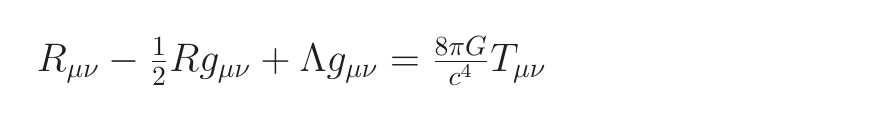
\begin{tikzpicture}
\node[textmain] at (-2,-4) {
\begin{minipage}{0.85\linewidth}
% \centering
\Large
$R_{\mu\nu} - \frac12Rg_{\mu\nu} + \Lambda g_{\mu\nu} = \frac{8\pi G}{c^4} T_{\mu\nu}$
\end{minipage}
};
% \draw[decorate,decoration={random steps,segment length=3pt,amplitude=0.5pt},white,very thin] 
%   (-1.8,1.7) -- (1.8,1.7);
\end{tikzpicture}
}

\switchcolumn

\begin{macterminal}[Skills]
$ vcastor.skills = {
~   "computational_chemistry_software" : [
~     "AMS (ADF,BAND,DFTB)", "Gaussian", "AIMAll", "Orca"
~   ],
~   "software_and_programming" : [
~     "UNIX-like OS", "Git §\color{terminalyellow}\faGit*§", "Subversion",
~     "Fortran", "§\color{terminalyellow}\LaTeX§", "Python §\color{terminalyellow}\faPython§", "SQL §\color{terminalyellow}\faDatabase§",
~     "C/C++", "perl"
~   ],
~   "gui_and_graphics" : [
~     "Inkscape", "GIMP", "tcl", "manim"
~   ],
~   "extras" : [
~     "Astrophysics", "First Aids"
~   ]
~ }
\end{macterminal}

% \vspace{-0.5cm}%
\hspace{2cm}\rotatebox{-3}{

\begin{tikzpicture}
\node[textmain] at (0,0) {
\begin{minipage}{0.85\linewidth}
\centering
\large
$(i\gamma^\mu\partial_\mu -m)\psi(x) = 0$
\end{minipage}
};
\draw[decorate,decoration={random steps,segment length=3pt,amplitude=0.5pt},textmain,very thin] 
  (-2.8,-0.7) -- (2.8,-0.7);
\end{tikzpicture}
}

\vspace{-0.3cm}%
\hspace{2cm}\rotatebox{4}{
\begin{tikzpicture}
\node[textmain] at (0,0) {
\begin{minipage}{0.85\linewidth}
\centering
\large
$\mathbf{F}\mathbf{C} = \mathbf{S}\mathbf{C}\varepsilon$
\end{minipage}
};
% \draw[decorate,decoration={random steps,segment length=3pt,amplitude=0.5pt},white,very thin] 
%   (-2.8,-0.7) -- (2.8,-0.7);
\end{tikzpicture}
}

\vspace{-2.4cm}%
\resizebox{0.16\textwidth}{!}{
\hspace{-1cm}\rotatebox{6}{
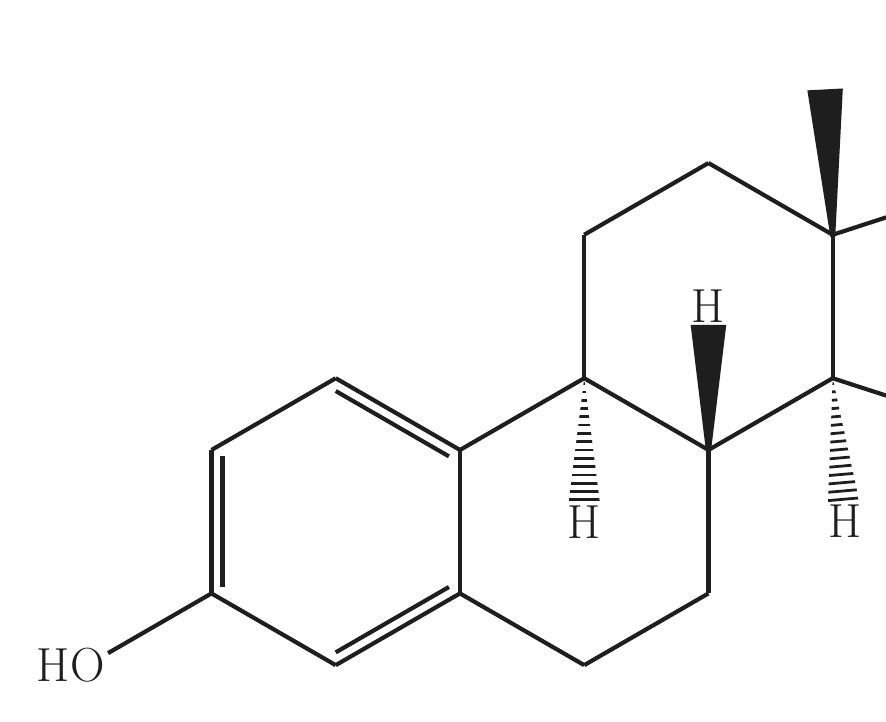
\begin{tikzpicture}
\node[textmain] at (0,0) {
\begin{minipage}{0.85\linewidth}
\centering
\LARGE
{\setchemfig{bond style={line width=1.5pt}, double bond sep=4pt, bond offset=1.5pt}
\chemfig{*6((-HO)-=*6(---([::-0]<H)*6(-([::-115]<:H)(*5(---(<OH)-([::-105]<)))----)-([::+120]<:H)-)-=-=)}
}
\end{minipage}
};
\end{tikzpicture}
}
}

\end{paracol}

% Magnetic field - absolute positioning
\AddToShipoutPictureBG*{%
\AtPageLowerLeft{%

\begin{tikzpicture}[remember picture, overlay, scale=1.0, >=latex, inner sep=0pt, outer sep=2pt,
    mark coordinate/.style={outer sep=0pt, minimum size=3pt, fill=textmain,circle}]
    
  \def\R{0.5}
  \def\angEl{30}
  \def\angAz{-140}
    
  \pgfmathsetmacro\H{\R*cos(\angEl)}
  \LongitudePlane[xzplane]{\angEl}{\angAz}
  \coordinate (O) at (4.5,4);
    
  \begin{scope}[shift={(O)}, rotate around={-15:(0,0)},
      field line/.style={color=terminalcyan, smooth, variable=\t, samples at={0,-5,-10,...,-360}}]
        
      \foreach \u in {0,-60,...,-120}{
        \LongitudePlane{\angEl}{\u}
        \foreach \r in {0.25,0.5,...,3.5} {
          \draw[current plane, field line] plot ({(\r)^2*(3*cos(\t)+cos(3*\t))}, 
                                                 {(\r)^2*(sin(\t)+sin(3*\t))});
        }
      }
      \foreach \u in {-240,-300}{
        \LongitudePlane{\angEl}{\u}
        \foreach \r in {0.25,0.5,...,3.5}{
          \draw[current plane, dashed, field line] plot ({(\r)^2*(3*cos(\t)+cos(3*\t))}, 
                                                         {(\r)^2*(sin(\t)+sin(3*\t))});
        }
      }
        
      \LongitudePlane[bzplane]{\angEl}{0}
      \foreach \r in {0.75,1.25,...,3.5}{
        \draw[bzplane, thick, field line] plot ({(\r)^2*(3*cos(\t)+cos(3*\t))}, 
                                                {(\r)^2*(sin(\t)+sin(3*\t))});
      }
        
      \fill[ball color=gray!40,opacity=0.4] (0,0) circle (\R);
      \draw[textmain] (0,0) circle (\R);
        
      \coordinate[mark coordinate] (Sm) at (0, \H);
      \coordinate[mark coordinate] (Nm) at (0,-\H);
      \path[xzplane] (Nm) -- +(0,-0.75) coordinate (Nm1) node[below,textmain] {$\mathbf{N}_m$}
                     (Sm) -- +(0,0.75) coordinate (Sm1) node[above,textmain] {$\mathbf{S}_m$};
    \draw[very thick, dashed, textmain] (Sm) -- (Nm);
    \draw[very thick, textmain] (Sm1) -- (Sm);
    \draw[very thick,->,>=latex', textmain] (Nm) -- (Nm1);
  \end{scope}
    
\end{tikzpicture}
}}

\end{document}

